\documentclass[twocolumn]{article}

\usepackage{scrextend}
\changefontsizes{8pt}

\makeatletter
\renewcommand*{\fps@figure}{!htb}
\renewcommand*{\fps@table}{!htb}
\makeatother

\usepackage{sectsty}
\sectionfont{\fontsize{11}{11}\selectfont}
\subsectionfont{\fontsize{10}{11}\selectfont}

% \usepackage[compact]{titlesec}
% \titlespacing{\section}{0pt}{2ex}{1ex}
% \titlespacing{\subsection}{0pt}{1ex}{1ex}
% \titlespacing{\subsubsection}{0pt}{0.5ex}{1ex}

\setlength{\parskip}{0cm}
\setlength{\parindent}{1em}

\usepackage{geometry}
 \geometry{
 a4paper,
 total={170mm,257mm},
 left=20mm,
 top=20mm,
 }
\usepackage[utf8]{inputenc}
\usepackage[hidelinks]{hyperref}
\usepackage{amsmath, bm}
\usepackage[ruled,vlined]{algorithm2e}
\usepackage{amssymb}
\usepackage{graphicx}
\usepackage{float}
\usepackage{booktabs}
\usepackage[parfill]{parskip}
\usepackage{comment}
\usepackage{subcaption}
\usepackage{booktabs}



\usepackage{listings}
\lstset{
    language=Python,
    breaklines=true,
    breakatwhitespace=true,
    basicstyle=\footnotesize,
    frame=lines
}
\usepackage[capitalise, nameinlink]{cleveref}

\usepackage[sorting=none, style=verbose]{biblatex}
\addbibresource{lab_3.bib}

\usepackage{titling}
\setlength{\droptitle}{-1cm}

\title{\Large COMP6248 Lab 3 Exercise -- Optimise it!}
\author{\small Wei Chien Teoh (Eugene)\\\bigskip \href{mailto:wct1c16@soton.ac.uk}{wct1c16@soton.ac.uk}}
\date{\small 29 April 2021}

\begin{document}

\maketitle

\section*{Introduction}

The results are seeded using \lstinline{torch.manual_seed(0)} to provide reproducible results.

\section{Exploring optimisation of analytic functions}

\subsection{Rastrigin}

\begin{figure}
    \centering
    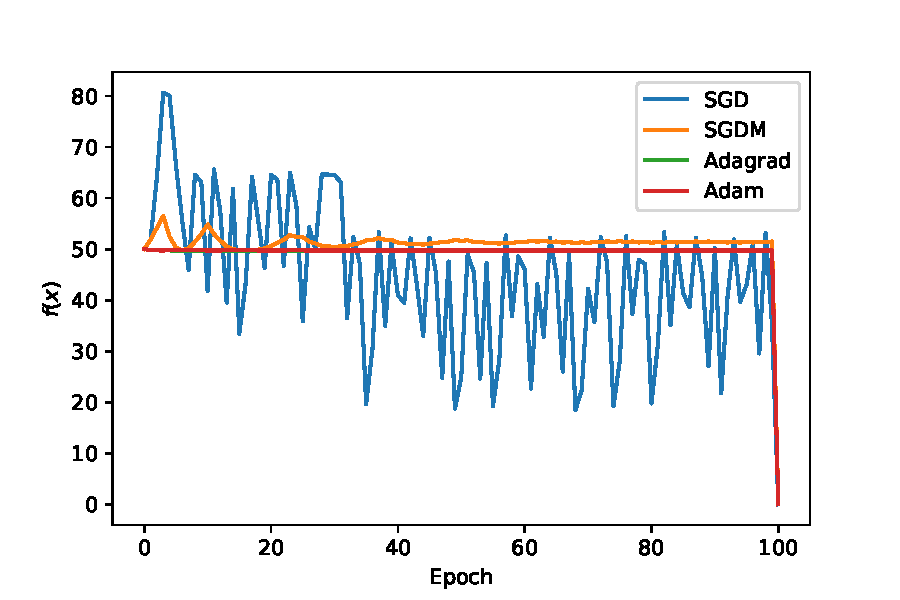
\includegraphics[width=\linewidth]{Figures/learning_curve.pdf}
    \caption{Learning curve for different optimisers.}
    \label{fig:learning-curve}
\end{figure}

\begin{figure}
    \centering
    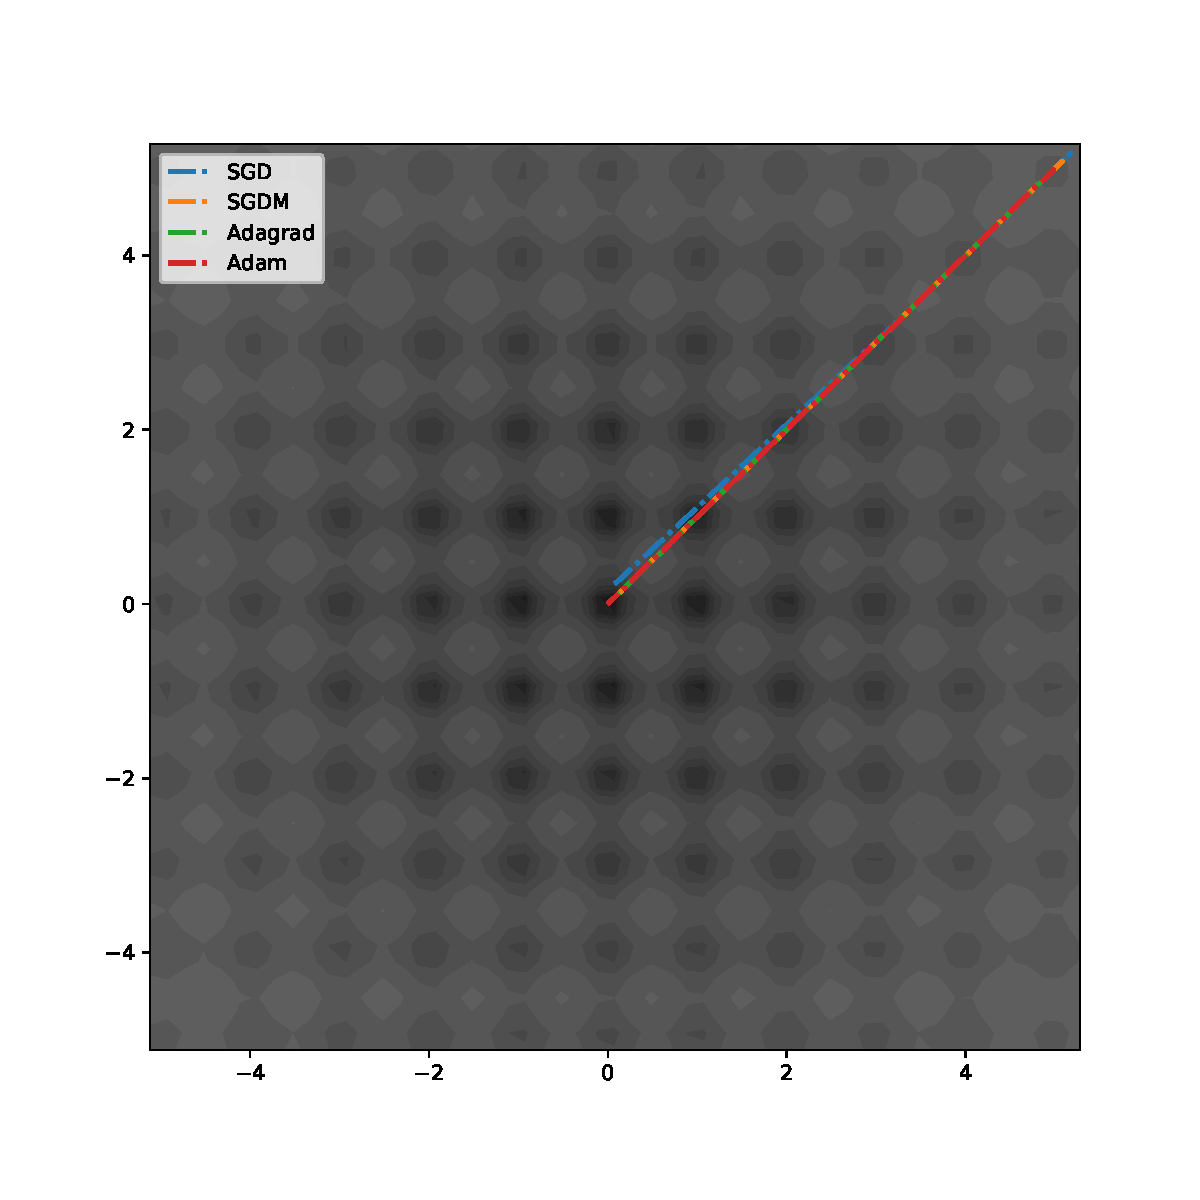
\includegraphics[width=\linewidth]{Figures/contour_plot.pdf}
    \caption{Contour plot and trajectory of different optimisers.}
    \label{fig:contour}
\end{figure}

\cref{fig:contour} shows all optimisers converge to the global minima at point (0, 0). All optimisers converge at around the same epoch, as illustrated in \cref{fig:learning-curve}. However, Adagrad and Adam, with identical performance, provide the most stability of between epochs. Hence, both are the best candidates for optimising the Rastrigin function.

\section{Optimisation of a SVM on real data}

\subsection{Iris SVM}

\cref{tab:acc} shows the mean and variance of accuracy after the SVM is repeatedly trained for 50 times with random initialisation of weights and biases. Both optimisers provide decent and close accuracies, with SGD slightly leading for both mean and variance. This is a surprising finding since the Adam optimiser was developed to improve upon SGD on various aspects such as speed of convergence. A potential explanation for this phenomenon is that adaptive optimisers such as Adam is observed to have worse generalisation than SGD despite it's better training performance \autocite{wilsonMarginalValueAdaptive2018}.

\begin{table}
    \centering
    \caption{Accuracy for 50 repeated experiments.}
    \label{tab:acc}
    \begin{tabular}{lrr}
    \toprule
    Optimiser &    Mean &  Variance \\
    \midrule
    SGD  &  0.9008 &  0.000399 \\
    Adam &  0.8912 &  0.000995 \\
    \bottomrule
    \end{tabular}
\end{table}


\end{document}